\uuid{7JVX}
\niveau{PCSI}
\module{Analyse}
\chapitre{Généralités sur les fonctions}
\sousChapitre{Études de fonctions}
%!TeX root=../../../encours.nouveau.tex
%%% Début exercice %%%

\duree{40}
\difficulte{1}
\auteur{Antoine Crouzet}
\datecreate{01/12/2024}
\titre{\'Etudes de fonctions}
\contenu{
\question{Etudier et représenter les fonctions suivantes :
\begin{align}
	f&:x\donne \frac{\eu{x}}{\eu{x}+1} & & &g&:x\donne x^{\frac{1}{x}}\\
	h&:x\donne \frac{\eu{x}+\eu{-x}}{2} & & &i&:x\donne \frac{x^3+x^2-2x-3}{2x^2-6}
\end{align}
On montrera que $i$ admet la droite d'équation $y=\frac{x+1}{2}$ pour asymptote au voisinage de $+\infty$ et $-\infty$.}
\reponse{\begin{align*}
$f$ est définie, continue et dérivable sur $\R$ comme quotient de fonctions dérivables ($\exp$) dont le dénominateur ne s'annule pas. On a :
\[ \lim_{x\rightarrow -\infty} \frac{\eu{x}}{\eu{x}+1} = 0 \quad\text{par quotient} \qeq \lim_{x\rightarrow +\infty} \frac{\eu{x}}{\eu{x}+1}=\lim_{x\rightarrow +\infty} \frac{1}{1+\eu{-x}} = 1 \quad \text{par quotient} \]
La courbe de $f$ admet donc deux asymptotes horizontales, une d'équation $y=0$ au voisinage de $-\infty$, et une d'équation $y=1$ au voisinage de $+\infty$.\\
Pour tout réel $x$,
\begin{eqnarray*}
	f'(x) &=& \frac{\eu{x}(\eu{x}+1) - \eu{x}(\eu{x})}{(\eu{x}+1)^2}\\
		  &=& \frac{\eu{x}}{(\eu{x}+1)^2}
\end{eqnarray*}
$f'$ est strictement positive sur $\R$, et donc $f$ est strictement croissante sur $\R$. On obtient le tableau de variations suivante :

\begin{center}
\begin{tikzpicture}
	 \tkzTabInit{$x$ / 1 , $f'(x)$ / 1, var de $f$ / 1.5}{$-\infty$, $+\infty$}
	 \tkzTabLine{, +,  }
	 \tkzTabVar{-/ $0$, +/ $1$}
\end{tikzpicture}
\end{center}
et la courbe représentative suivante :
\begin{center}
	\input{fig.ex2}
\end{center}
$g : x \donne \eu{\frac{1}{x}\ln(x)}$ est définie et dérivable sur $\R^*_+$ comme composée de la fonction $x\donne \frac{\ln(x)}{x}$ et de l'exponentielle. \\
Par quotient, $\ds{\lim_{x\rightarrow 0^+} \frac{\ln(x)}{x} = -\infty}$. Par composée, \[ \lim_{x\rightarrow +\infty} g(x)=0 \]
De même, par croissance comparée, $\ds{\lim_{x\rightarrow +\infty} \frac{\ln(x)}{x} = 0}$. Par composée,  \[ \lim_{x\rightarrow +\infty} g(x)=1 \]
Pour tout réel $x>0$, on pose $\ds{u(x)=\frac{\ln(x)}{x}}$. Par quotient,
\[ u'(x) = \frac{\frac{1}{x}x-\ln(x)(1)}{x^2}=\frac{1-\ln(x)}{x^2} \]
et par composée :
 \begin{eqnarray*}
 	g'(x) &=& u'(x) \eu{u(x)} \\
 		  &=& \frac{1-\ln(x)}{x^2} \eu{\frac{\ln(x)}{x}}
 \end{eqnarray*}
 Puisque pour tout $x>0$, $\ds{\eu{\frac{\ln(x)}{x}}>0}$, $g'$ est du signe de $\ds{\frac{1-\ln(x)}{x^2}}$, donc de $1-\ln(x)$. Or
 \begin{eqnarray*}
 	1-\ln(x) > 0 &\Leftrightarrow& 1> \ln(x) \\ &\Leftrightarrow& \E > x \quad \text{par stricte croissance de $\ln$}
 \end{eqnarray*}
 avec $\ds{g(\E) = \eu{\frac{\ln(\E)}{\E}} = \E^\frac{1}{\E}}$.
Ainsi, on dispose du tableau de variation suivant :
\begin{center}
\begin{tikzpicture}
	 \tkzTabInit{$x$ / 1 , $g'(x)$ / 1, var de $g$ / 1.5}{$0$, $\E$, $+\infty$}
	 \tkzTabLine{d, +, z, -, }
	 \tkzTabVar{D-/ $0$, +/ $\eu{\frac{1}{\E}}$, -/ $1$}
\end{tikzpicture}
\end{center}
et de la courbe représentative suivante :
\begin{center}
	\input{fig.ex3}
\end{center}
$h$ est définie et dérivable sur $\R$ par somme de deux fonctions dérivables. Sa dérivée est \[ h':x\mapsto \frac{\eu{x}-\eu{-x}}{2} \]
dont le signe est, en utilisant la croissance de la fonction $\ln$ :
\[ \eu{x}-\eu{-x}\geq 0 \iff \eu{x}\geq \eu{-x}\iff x\geq -x \iff x\geq 0. \]
Par somme et produit \[ \lim_{x\to -\infty} h(x) =\lim_{x\to +\infty} h(x) = +\infty. \]
On obtient le tableau suivant :
\begin{center}
	\begin{tikzpicture}
	   \tkzTabInit{$x$ / 1 , $h'(x)$ / 1, $h(x)$ / 1.5}{$-\infty$, $0$, $+\infty$}
	   \tkzTabLine{, -, z, +, }
	   \tkzTabVar{+/ $+\infty$, -/ $1$, +/ $+\infty$}
	\end{tikzpicture}
\end{center}
et la courbe représentative :

Enfin, $i$ est définie sur $\R \setminus \left \{ -\sqrt{3}, \, \sqrt{3} \right \}$ et y est dérivable. Par factorisation classique :
\[ \lim_{x\to -\infty} i(x)= -\infty \qeq \lim_{x\to +\infty} i(x)=+\infty. \]
Enfin, \[ \lim_{x\to (\sqrt{3})^+} 2x^2-6= 0^+,\quad \lim_{x\to (\sqrt{3})^-} 2x^2-6= 0^-, \lim_{x\to (-\sqrt{3})^+} 2x^2-6= 0^-,\quad \lim_{x\to (-\sqrt{3})^-} 2x^2-6= 0^+ , \]
et
\[ \lim_{x\to \sqrt{3}} x^3+x^2-2x-3=\sqrt{3} \qeq \lim_{x\to -\sqrt{3}} x^3+x^2-2x-3=-\sqrt{3}. \]
et par quotient :
\[ \lim_{x\to (-\sqrt{3})^-} i(x) = -\infty,\quad \lim_{x\to (-\sqrt{3})^+} i(x) = +\infty,\quad \lim_{x\to (\sqrt{3})^-} i(x) = -\infty,\qeq \lim_{x\to (\sqrt{3})^+} i(x) = +\infty\]
La dérivée de $i$ est
\[ x\donne \frac{(3x^2+2x-2)(2x^2-6)-(x^3+x^2-2x-3)(4x)}{(2x^2-6)^2} = \frac{2(x^4-7x^2+6)}{(2x^2-6)^2} \]

On déterminer le signe de $x^4-7x^2+6$ par la méthode classique. On pose $X=x^2$. Les solutions de $X^2-7X+6$ sont $6$ et $1$. On peut alors écrire
\[ X^4-7X^2+6 = (X-1)(X+1)(X-\sqrt{6})(X+\sqrt{6}). \]
Le tableau de signe est alors
\begin{center}
	\begin{tikzpicture}
	   \tkzTabInit[lgt = 2.5, espcl = 2]{$x$ / 1 , $X^4-7X^2+6$ / 1}{$-\infty$, $-\sqrt{6}$, $-1$, $1$, $\sqrt{6}$, $+\infty$}
	   \tkzTabLine{ , +, z, -, z, +, z, -, z, +, }
	\end{tikzpicture}
\end{center}
On en déduit le tableau de variations suivant :
\begin{center}
	\begin{tikzpicture}
	   \tkzTabInit[lgt = 2, espcl = 2]{$x$ / 1 , $i(x)$ / 1, var de $i$ / 2}{$-\infty$, $-\sqrt{6}$, $-\sqrt{3}$, $-1$, $1$, $\sqrt{3}$, $\sqrt{6}$, $+\infty$}
	   \tkzTabLine{ , +, z, -, d, -, z, +, z, -, d, -, z, +, }
		 \tkzTabVar{- / $-\infty$, + / $\frac{3-4\sqrt{6}}{6}$, -D+/ $-\infty$ / $+\infty$, - / $\frac14$, + / $\frac34$, -D+ / $-\infty$ / $+\infty$, -/$\frac{3+4\sqrt{6}}{6}$, + / $+\infty$ }
	\end{tikzpicture}
\end{center}
\end{align*}}
}

%%% Fin exercice %%%
